%%%%%%%%%%%%%%%%%%%%%%%%%%%%%%%%%%%%%%%%%
% Short Sectioned Assignment
% LaTeX Template
% Version 1.0 (5/5/12)
%
% This template has been downloaded from:
% http://www.LaTeXTemplates.com
%
% Original author:
% Frits Wenneker (http://www.howtotex.com)
%
% License:
% CC BY-NC-SA 3.0 (http://creativecommons.org/licenses/by-nc-sa/3.0/)
%
%%%%%%%%%%%%%%%%%%%%%%%%%%%%%%%%%%%%%%%%%

%----------------------------------------------------------------------------------------
%	PACKAGES AND OTHER DOCUMENT CONFIGURATIONS
%----------------------------------------------------------------------------------------

\documentclass{article} % A4 paper and 11pt font size

\usepackage[T1]{fontenc} % Use 8-bit encoding that has 256 glyphs
\usepackage[english]{babel} % English language/hyphenation
\usepackage{amsmath} % Math packages
\usepackage{enumerate}
\usepackage{algpseudocode}
\usepackage{graphicx}

\usepackage{fancyhdr} % Custom headers and footers
\pagestyle{fancyplain} % Makes all pages in the document conform to the custom headers and footers
\fancyhead{} % No page header - if you want one, create it in the same way as the footers below
\fancyfoot[L]{} % Empty left footer
\fancyfoot[C]{} % Empty center footer
\fancyfoot[R]{\thepage} % Page numbering for right footer
\setlength{\headheight}{13.6pt} % Customize the height of the header
\renewcommand{\headrulewidth}{0pt} % Remove header underlines
\renewcommand{\footrulewidth}{0pt} % Remove footer underlines

\allowdisplaybreaks

% Margins
\topmargin=-0.8in
\evensidemargin=0in
\oddsidemargin=0in
\textwidth=6.5in
\textheight=9.0in
\headsep=0.5in

%----------------------------------------------------------------------------------------
%	TITLE SECTION
%----------------------------------------------------------------------------------------

\newcommand{\horrule}[1]{\rule{\linewidth}{#1}} % Create horizontal rule command with 1 argument of height

\title{
\normalfont \normalsize
\textsc{University of Toronto} \\ [25pt] % Your university, school and/or department name(s)
\horrule{0.5pt} \\[0.4cm] % Thin top horizontal rule
\huge CSC418 Assignment 1 Part A \\ % The assignment title
\horrule{2pt} \\[0.5cm] % Thick bottom horizontal rule
}

\author{Nicholas Dujay\\999194900} % Your name

\date{\normalsize\today} % Today's date or a custom date

\begin{document}

\maketitle % Print the title

%----------------------------------------------------------------------------------------
%	PROBLEM 1
%----------------------------------------------------------------------------------------

\section{Question 1}
Given that $\vec{e} = (1,2,2)$ $\vec{g} =(1,1,3)$ and $\vec{r}=(0,1,0)$, $\vec{s}$ $\vec{u}$ and $\vec{v}$ are calculated like this:

\begin{align*}
\vec{s}&=-\frac{\vec{g}}{\| \vec{g} \|} = \left(-\frac{1}{\sqrt{11}},-\frac{1}{\sqrt{11}},-\frac{3}{\sqrt{11}} \right) \\
\vec{u}&=\frac{\vec{r} \times \vec{s}}{\|\vec{r} \times \vec{s}\|} = \left(-\frac{3}{\sqrt{10}},0,\frac{1}{\sqrt{10}} \right)\\
\vec{v}&=\frac{\vec{s} \times \vec{u}}{\|\vec{s} \times \vec{u}\|} = \left(-\frac{1}{\sqrt{110}},\sqrt{\frac{10}{11}},-\frac{3}{\sqrt{110}} \right)
\end{align*}

From here, we can calculate the world to camera transformation matrix as follows:
\begin{align*}
M_{wc} &= \left[
\begin{array}{ccc|c}
-\frac{3}{\sqrt{10}} & 0 & \frac{1}{\sqrt{10}}  & \frac{1}{\sqrt{10}}\\
-\frac{1}{\sqrt{110}} & \sqrt{\frac{10}{11}} & -\frac{3}{\sqrt{110}} & -\frac{13}{\sqrt{110}}\\
-\frac{1}{\sqrt{11}} & -\frac{1}{\sqrt{11}} & -\frac{3}{\sqrt{11}} & \frac{9}{\sqrt{11}}\\
0 & 0 & 0 & 1
\end{array}
\right]\\
&\text{Where the $M_{wc}$ matrix has the following form:}\\
M_{wc} &= \left[
\begin{array}{ccc|c}
u_x & u_y & u_z & -\vec{u} \cdot \vec{e} \\
v_x & v_y & v_z & -\vec{v} \cdot \vec{e} \\
s_x & s_y & s_z & -\vec{s} \cdot \vec{e} \\
0 & 0 & 0 & 1
\end{array}
\right]
\end{align*}

%----------------------------------------------------------------------------------------
%	PROBLEM 2
%----------------------------------------------------------------------------------------
\section{Question 2}
First lets calculate $m$ then project it to $m'$.
\begin{align*}
m &= \frac{1}{2} \left(p+q\right)=\frac{1}{2}\left(
\begin{bmatrix}
p_x\\
p_y\\
p_z\\
1
\end{bmatrix}
+
\begin{bmatrix}
q_x\\
q_y\\
q_z\\
1
\end{bmatrix}
\right)
= \begin{bmatrix}
\frac{1}{2}(p_x + q_x)\\
\frac{1}{2}(p_y + q_y)\\
\frac{1}{2}(p_z + q_z)\\
1
\end{bmatrix}\\
m' &=
\begin{bmatrix}
1 & 0 & 0 & 0\\
0 & 1 & 0 & 0\\
0 & 0 & 1 & 0\\
0 & 0 & -\frac{1}{f} & 0\\
\end{bmatrix}
\cdot
\begin{bmatrix}
\frac{1}{2}(p_x + q_x)\\
\frac{1}{2}(p_y + q_y)\\
\frac{1}{2}(p_z + q_z)\\
1
\end{bmatrix}
\cong \begin{bmatrix}
-f\left(\frac{p_x + q_x}{p_z + q_z}\right)\\
-f\left(\frac{p_y + q_y}{p_z + q_z}\right)\\
-f\\
1
\end{bmatrix}
\end{align*}


Next lets calculate $p'$ and $q'$ then calculate the midpoint between them.
\begin{align*}
p' &=
\begin{bmatrix}
1 & 0 & 0 & 0\\
0 & 1 & 0 & 0\\
0 & 0 & 1 & 0\\
0 & 0 & -\frac{1}{f} & 0\\
\end{bmatrix}
\cdot
\begin{bmatrix}
p_x\\
p_y\\
p_z\\
1
\end{bmatrix}
\cong
\begin{bmatrix}
-f\frac{p_x}{p_z}\\
-f\frac{p_y}{p_z}\\
-f\\
1
\end{bmatrix}\\
&\text{$q'$ is calculated similarly.}\\
\frac{1}{2}\left(p'+q'\right) &=
\frac{1}{2}
\left(
\begin{bmatrix}
-f\frac{p_x}{p_z}\\
-f\frac{p_y}{p_z}\\
-f\\
1
\end{bmatrix}
+
\begin{bmatrix}
-f\frac{q_x}{q_z}\\
-f\frac{q_y}{q_z}\\
-f\\
1
\end{bmatrix}
\right)
\cong
\begin{bmatrix}
-\frac{f}{2}\left(\frac{p_x}{p_z} + \frac{q_x}{q_z}\right)\\
-\frac{f}{2}\left(\frac{p_y}{p_z} + \frac{q_y}{q_z}\right)\\
-f\\
1
\end{bmatrix}
\end{align*}
In order for $m' = \frac{1}{2}(p'+q')$, we need $-f\left(\frac{p_x + q_x}{p_z + q_z}\right) = -\frac{f}{2}\left(\frac{p_x}{p_z} + \frac{q_x}{q_z}\right)$ and $-f\left(\frac{p_y + q_y}{p_z + q_z}\right) = -\frac{f}{2}\left(\frac{p_y}{p_z} + \frac{q_y}{q_z}\right)$. There's only one case where this is true, and it is when $p_z = q_z$.
\\
If we instead use an orthographic projection, then $m' = \frac{1}{2}(p'+q')$ for all cases:
\begin{align*}
m' &=
\begin{bmatrix}
1 & 0 & 0 & 0\\
0 & 1 & 0 & 0\\
0 & 0 & 0 & 1\\
\end{bmatrix}
\cdot
\begin{bmatrix}
\frac{1}{2}(p_x + q_x)\\
\frac{1}{2}(p_y + q_y)\\
\frac{1}{2}(p_z + q_z)\\
1
\end{bmatrix}
=
\begin{bmatrix}
\frac{1}{2}(p_x + q_x)\\
\frac{1}{2}(p_y + q_y)\\
1
\end{bmatrix}\\
p' &=
\begin{bmatrix}
1 & 0 & 0 & 0\\
0 & 1 & 0 & 0\\
0 & 0 & 0 & 1\\
\end{bmatrix}
\cdot
\begin{bmatrix}
p_x\\
p_y\\
p_z\\
1
\end{bmatrix} = \begin{bmatrix}
p_x\\
p_y\\
1
\end{bmatrix}\\
\frac{1}{2}\left(p' + q'\right) &=
\frac{1}{2}
\left(
\begin{bmatrix}
p_x\\
p_y\\
1
\end{bmatrix}
+
\begin{bmatrix}
q_x\\
q_y\\
1
\end{bmatrix}
\right)\\
&=
\begin{bmatrix}
\frac{1}{2}(p_x + q_x)\\
\frac{1}{2}(p_y + q_y)\\
1
\end{bmatrix}= m'
\end{align*}

%----------------------------------------------------------------------------------------
%	PROBLEM 3
%----------------------------------------------------------------------------------------
\section{Question 3}

The projected lines have the following form
\begin{align*}
l_i(u_i)' =
\begin{bmatrix}
1 & 0 & 0 & 0\\
0 & 1 & 0 & 0\\
0 & 0 & 1 & 0\\
0 & 0 & \frac{1}{f} & 0\\
\end{bmatrix}
\cdot
\begin{bmatrix}
p_{ix} + u_i d_{ix}\\
p_{iy} + u_i d_{iy}\\
p_{iz} + u_i d_{iz}\\
1
\end{bmatrix}
=
\begin{bmatrix}
p_{ix} + u_i d_{ix}\\
p_{iy} + u_i d_{iy}\\
p_{iz} + u_i d_{iz}\\
\frac{1}{f} \left(p_{iz} + u_i d_{iz}\right)
\end{bmatrix}
\cong
\begin{bmatrix}
f\frac{p_{ix} + u_i d_{ix}}{p_{iz} + u_i d_{iz}}\\
f\frac{p_{iy} + u_i d_{iy}}{p_{iz} + u_i d_{iz}}\\
f\\
1
\end{bmatrix}
\end{align*}

The projection of each line will intersect in the canonical view space, so the final expression is independent of the original lines. However, since the original lines never intersect in camera space, the point of intersection is at $u_i = \pm\infty$. Therefore, we must take the limit of $l_i'(u_i)$ as $u_i \to \pm \infty$.
\begin{align*}
\lim_{u_i \to \pm \infty} l_i(u_i) &=
\lim_{u_i \to \pm \infty}  \begin{bmatrix}
f\frac{p_{ix} + u_i d_{ix}}{p_{iz} + u_i d_{iz}}\\
f\frac{p_{iy} + u_i d_{iy}}{p_{iz} + u_i d_{iz}}\\
f\\
1
\end{bmatrix}
= \begin{bmatrix}
\lim_{u_i \to \pm \infty} f\frac{p_{ix} + u_i d_{ix}}{p_{iz} + u_i d_{iz}}\\
\lim_{u_i \to \pm \infty} f\frac{p_{iy} + u_i d_{iy}}{p_{iz} + u_i d_{iz}}\\
f\\
1
\end{bmatrix}\\
&= \begin{bmatrix}
\lim_{u_i \to \pm \infty} f\frac{p_{ix} + u_i d_{ix}}{\frac{p_{iz}}{u_i} + d_{iz}}\\
\lim_{u_i \to \pm \infty} f\frac{p_{iy} + u_i d_{iy}}{\frac{p_{iz}}{u_i} + d_{iz}}\\
f\\
1
\end{bmatrix}
= \begin{bmatrix}
\lim_{u_i \to \pm \infty} f\frac{\frac{p_{ix}}{u_i} + d_{ix}}{\frac{p_{iz}}{u_i} + d_{iz}}\\
\lim_{u_i \to \pm \infty} f\frac{\frac{p_{iy}}{u_i} + d_{iy}}{\frac{p_{iz}}{u_i} + d_{iz}}\\
f\\
1
\end{bmatrix}\\
&= \begin{bmatrix}
f\frac{d_{ix}}{d_{iz}}\\
f\frac{d_{iy}}{d_{iz}}\\
f\\
1
\end{bmatrix}
\end{align*}
%----------------------------------------------------------------------------------------

%----------------------------------------------------------------------------------------
%	PROBLEM 4
%----------------------------------------------------------------------------------------

\section{Question 4}
The canonical view transform using $L=-1, R = 1, B = -1, T = 1, f = 1, F=1001$ is this:
\begin{align*}
M_{cv} &=
\begin{bmatrix}
\frac{2f}{L-R} & 0 & \frac{R + L}{L - R} & 0\\
0 & \frac{2f}{B-T} & \frac{B + T}{B - T} & 0\\
0 & 0 & \frac{f + F}{F - f} & \frac{2Ff}{F - f}\\
0 & 0 & -\frac{1}{f} & 0\\
\end{bmatrix}
= \begin{bmatrix}
\frac{2}{-1-1} & 0 & \frac{1 + -1}{-1 - 1} & 0\\
0 & \frac{2}{-1-1} & \frac{-1 + 1}{-1 - 1} & 0\\
0 & 0 & \frac{1 + 1001}{1001 - 1} & \frac{2(1001)}{1001 - 1}\\
0 & 0 & -\frac{1}{f} & 0\\
\end{bmatrix}
=
\begin{bmatrix}
-1 & 0 & 0 & 0\\
0 & -1 & 0 & 0\\
0 & 0 & 1.002 & 2.002\\
0 & 0 & -1 & 0\\
\end{bmatrix}\\
&\text{Now transforming a point from camera space to canonical view space:}\\
\begin{bmatrix}
x_v\\
y_v\\
z_v\\
1\\
\end{bmatrix}
&= M_{cv} \begin{bmatrix}
x_c\\
y_c\\
z_c\\
1\\
\end{bmatrix}
= \begin{bmatrix}
-x_c\\
-y_c\\
1.002 z_c + 2.002\\
z_c\\
\end{bmatrix}
\cong
\begin{bmatrix}
-\frac{x_c}{z_c}\\
-\frac{y_c}{z_c}\\
1.002 + \frac{2.002}{z_c}\\
1\\
\end{bmatrix}
\end{align*}
Since we are only interested in the pseudo depth value here, we now have a formula for the pseudo depth of each point.
$z_{c1}=-1, z_{c2}=-10, z_{c3} = -100, z_{c4} = -1000$
\begin{align*}
z_{v1} &= 1.002 + \frac{2.002}{z_{c1}} = -1\\
z_{v2} &= 1.002 + \frac{2.002}{z_{c2}} = 0.8018\\
z_{v3} &= 1.002 + \frac{2.002}{z_{c3}} = 0.98198\\
z_{v4} &= 1.002 + \frac{2.002}{z_{c4}} = 0.999998\\
\end{align*}

The relationship is not linear. Plot $z_{ci}$ and $z_{vi}$ on a graph and calculate slopes between each pair of points $(-1, -1), (-10, 0.8018), (-100, 0.98198), (-1000, 0.999998)$ and the slopes between each point should be the same if the relationship is linear. However, the slopes are different between each point so therefore the relationship is not linear.
%----------------------------------------------------------------------------------------

%----------------------------------------------------------------------------------------
%	PROBLEM 5
%----------------------------------------------------------------------------------------

\section{Question 5}
\begin{enumerate}[a)]

\item
The general equation of an ellipse in 2d is $x(t) = cos(t), y(t) = sin(t)$, for some $t \in [0,n]$. In the $xy$-plane we must hold hold $u$ constant since $t$ is the planar parameter of the equation. Similarly for the cross section of the ellipsoid and the $x=0$ plane, we must hold $t$ constant.
\\
\\
\begin{minipage}{0.45\textwidth}
Let $u=\frac{1}{4}$. The equation of the ellipse that is the cross section of the ellipsoid and the plane $z=0$ is given by $e_1(t)$.
\begin{eqnarray*}
x(t) &=& x\left(t, \frac{1}{4}\right) = a \cos(2\pi t) \sin\left(\frac{\pi}{2}\right) = a \cos (2 \pi t)\\
y(t) &=& y\left(t,\frac{1}{4}\right) = b \sin (2 \pi t) \sin\left(\frac{\pi}{2}\right) = b \sin (2 \pi t)\\
z(t) &=& z\left(t,\frac{1}{4}\right) = 0\\
e_1(t) &=& \left(a \cos (2 \pi t), b \sin (2 \pi t), 0\right)
\end{eqnarray*}
\end{minipage}\
\quad\quad\quad\quad\quad
\begin{minipage}{0.45\textwidth}
Let $t=\frac{1}{4}$. The equation of the ellipse that is the cross section of the ellipsoid and the plane $x=0$ is given by $e_2(t)$.
\begin{eqnarray*}
x(u) &=& x\left(\frac{1}{4},u\right) = a \cos\left(\frac{\pi}{2}\right) \sin(2 \pi u) = 0\\
y(u) &=& y\left(\frac{1}{4},u\right) = b \sin \left(\frac{\pi}{2}\right) \sin(2 \pi u) = b \sin (2 \pi u)\\
z(u) &=& z\left(\frac{1}{4},u\right) = c \cos(2 \pi u)\\
e_2(u) &=& \left(0, b \sin (2 \pi u), c \cos(2 \pi u)\right)
\end{eqnarray*}
\end{minipage}

\item
The tangent to these ellipses are simply the derivative of their equations.
\begin{eqnarray*}
\frac{\delta e_1(t)}{\delta t} &=& \left(a \cos (2 \pi t), b \sin (2 \pi t), 0\right) = \left(-a 2 \pi \sin (2 \pi t), b 2 \pi \cos (2 \pi t), 0\right)\\
\frac{\delta e_2(u)}{\delta u} &=& \left(0, b \sin (2 \pi u), c \cos(2 \pi u)\right) = \left(0, b 2 \pi \cos (2 \pi u), - c 2 \pi \sin (2 \pi u)\right)
\end{eqnarray*}

The normal to the ellipses is the cross product of these two tangent vectors.
\begin{eqnarray*}
\frac{\delta e_1(t)}{\delta t} \times \frac{\delta e_2(u)}{\delta u} &=& (-4 \pi^2 b c \cos(2 \pi t) \sin (2 \pi u), -4 \pi^2 a c \sin(2 \pi t) \sin (2 \pi u), -4 \pi^2 a b \sin(2 \pi t) \cos (2 \pi u))\\
&=& -4 \pi^2 a b c \left(\frac{\cos(2 \pi t) \sin (2 \pi u)}{a}, \frac{\sin(2 \pi t) \sin (2 \pi u)}{b}, \frac{\sin(2 \pi t) \cos (2 \pi u)}{c}\right)
\end{eqnarray*}

However, these normals are only valid when $e_1(t) = e_2(u)$. Setting $e_1(t) = e_2(u)$ and solving for $t$ and $u$, we get $t=u$ and $t=\frac{1}{4}, \frac{3}{4}$. Subbing in these values of $t$ and $u$, we get the final expression for the normal to be: $-4 \pi^2 a b c (0, \frac{1}{b}, 0)$, and $4 \pi^2 a b c (0, \frac{1}{b}, 0)$ (for the other side). 


\item
First, lets find $x^2$, $y^2$, $z^2$.
\begin{eqnarray*}
x^2 &= (a \cos (2 \pi t) \sin(2 \pi u))^2 =& a^2 \cos^2(2 \pi t) \sin^2 (2 \pi u)\\
y^2 &= (b \sin (2 \pi t) \sin(2 \pi u))^2 =& b^2 \sin^2(2 \pi t) \sin^2 (2 \pi u)\\
z^2 &= (c \cos (2 \pi u))^2 =& c^2 \cos^2(2 \pi u)\\
\end{eqnarray*}

Then lets calculate $\frac{x^2}{a^2} + \frac{y^2}{b^2} + \frac{z^2}{c^2}$.

\begin{eqnarray*}
\frac{x^2}{a^2} + \frac{y^2}{b^2} + \frac{z^2}{c^2} &=& \frac{a^2 \cos^2(2 \pi t) \sin^2 (2 \pi u)}{a^2} +  \frac{b^2 \sin^2(2 \pi t) \sin^2 (2 \pi u)}{b^2} + \frac{c^2 \cos^2(2 \pi u)}{c^2}\\
&=& \cos^2(2 \pi t) \sin^2 (2 \pi u) +  \sin^2(2 \pi t) \sin^2 (2 \pi u) + \cos^2(2 \pi u)\\
&=& \sin^2 (2 \pi u)(\cos^2(2 \pi t) +  \sin^2(2 \pi t))+ \cos^2(2 \pi u)\\
&=& \sin^2 (2 \pi u) + \cos^2(2 \pi u)\\
&=& 1
\end{eqnarray*}

Therefore, the implicit equation of a ellipsoid is $\frac{x^2}{a^2} + \frac{y^2}{b^2} + \frac{z^2}{c^2} = 1$.

\item
The normal to a point on the ellipse is simply the gradient of the equation derived in part c.
\begin{align*}
\nabla f(x,y,z) &= \left(\frac{\partial f}{\partial x},\frac{\partial f}{\partial y},\frac{\partial f}{\partial z}\right)\\
&= \left(\frac{2x}{a^2},\frac{2y}{b^2},\frac{2z}{c^2}\right)\\
&\text{If we sub in $x(t,u)$ for $x$, (and similarly for $y$ and $z$) then we get the normal vector in terms of $t,u$}\\
&= 2 \left(\frac{\cos(2 \pi t) \sin(2 \pi u)}{a},\frac{\sin(2 \pi t) \sin(2 \pi u)}{b},\frac{\cos(2 \pi u)}{c}\right)\\
\end{align*}

\end{enumerate}

%----------------------------------------------------------------------------------------

%----------------------------------------------------------------------------------------
%	PROBLEM 6
%----------------------------------------------------------------------------------------

\section{Question 6}
\begin{figure}[h!]
\centering
	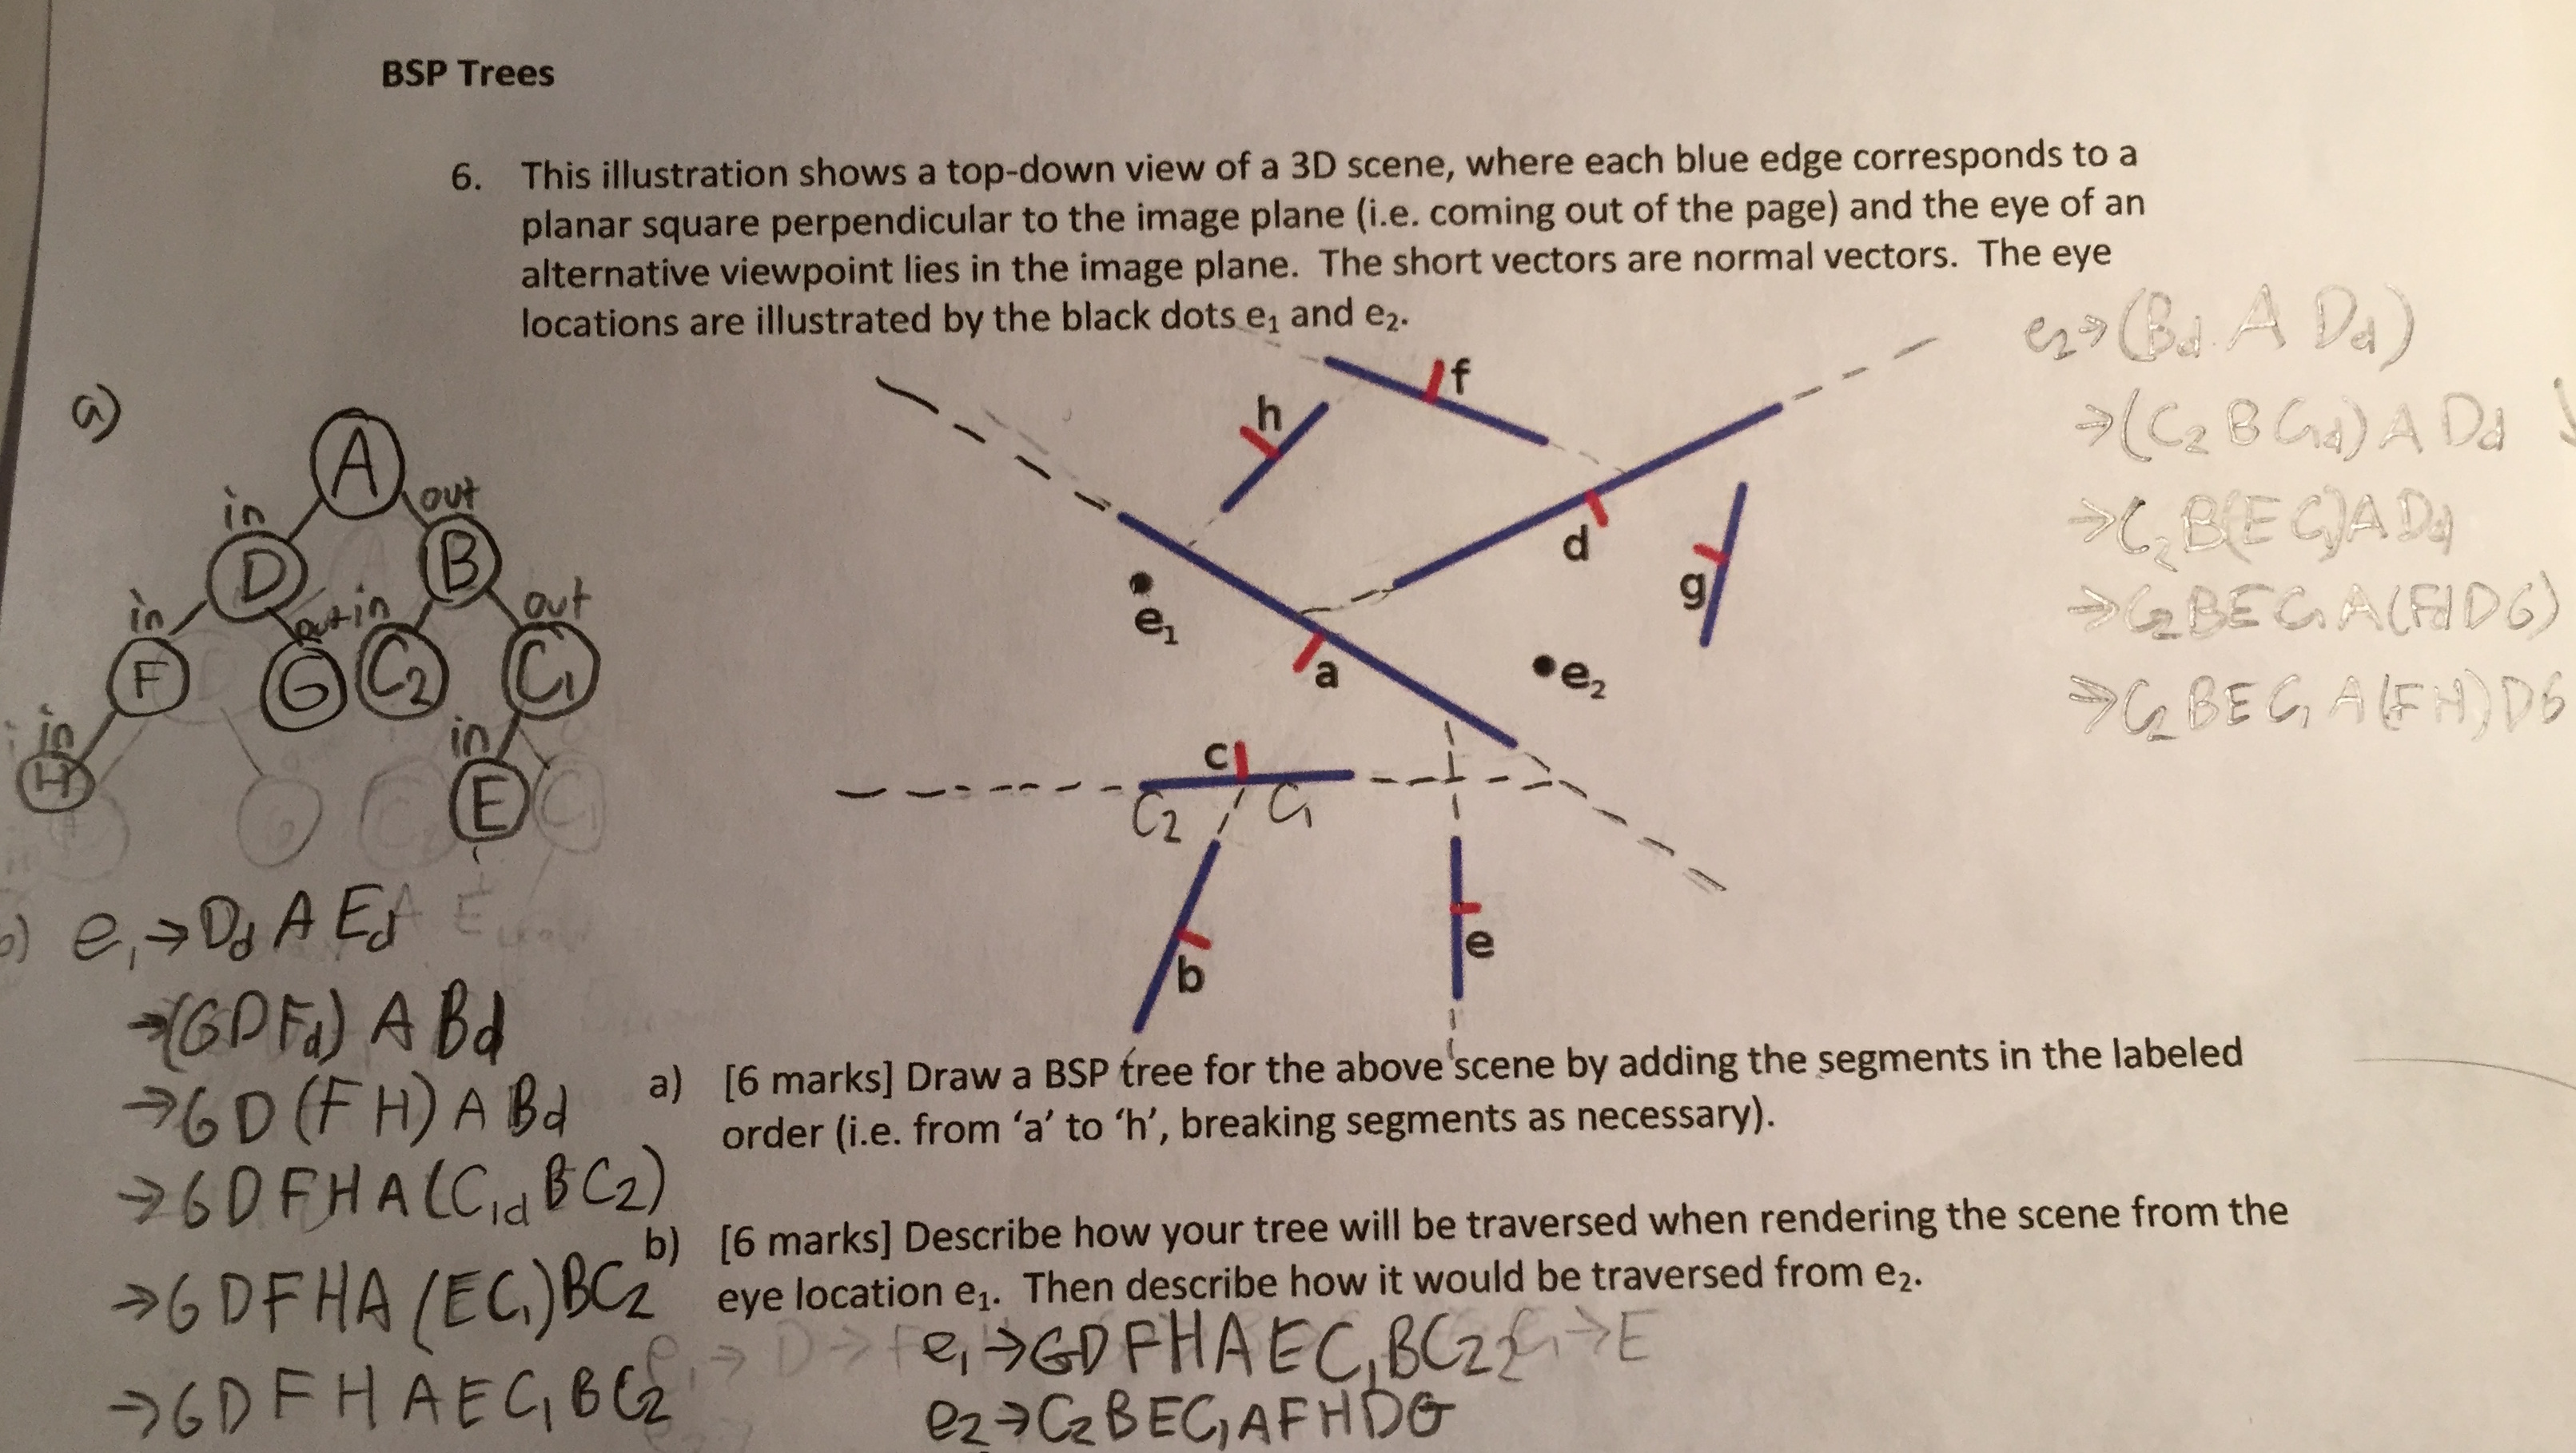
\includegraphics[width=\textwidth]{q6}
\end{figure}
%----------------------------------------------------------------------------------------
\end{document}
